\documentclass[10pt]{article}
\usepackage[top=1cm, bottom=1cm, left=1cm, right=1cm]{geometry}
\usepackage{graphicx}
\usepackage{multicol}
\usepackage[colorlinks=true]{hyperref}
\usepackage{verbatim}
\usepackage{enumerate}
\usepackage{wrapfig} 

\title{Wesnoth UMC Development \\ Developer's Manual}
\author{Timotei Dolean - \href{mailto:timotei21@gmail.com}{timotei21@gmail.com}}

\begin{document}

\maketitle

\tableofcontents
\setcounter{tocdepth}{3}
\newpage

\newcounter{cnt}
\newcommand{\icnt}{ \stepcounter{cnt} \thecnt }

\section{Foreword}
\begin{multicols}{2}
  \begin{center}
    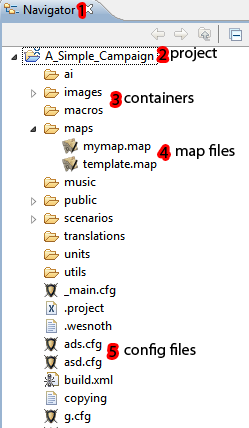
\includegraphics[scale=0.6]{definitions.png}
  \end{center}
Through this readme the following terms with the specified meaning will be used:
\begin{enumerate}
\item Navigator / Project Explorer / Package Explorer - an Eclipse view that shows the projects in the workspace
\item Project - a directory on the harddrive that is represented as a top directory in the navigator.
\item Container - this is a directory or a project. Basically it can contain any file or directory children.
\end{enumerate}

The following image will highlight the terms used: 1 - Navigator, 2 - Project, 3 - Containers, 4 - Map files, 5 - Config files that contain WML code
\end{multicols}

\section{Prerequisites}
A quick list before getting into details:
\begin{enumerate}
\item Java 6
\item Python 2.x
\item Eclipse 3.5 or newer
\item Wesnoth 1.9.x, trunk or newer
\end{enumerate}

Now for getting all those items:
\begin{enumerate}
\item The plugin runs on the following platforms: Windows 32/64 bit, Linux 32/64 bit and Mac OSX 64bit. Note that \textbf{Mac OSX 32 bit} is \textbf{not supported}. If you want to know why, please consult the Frequently Asked Questions section.
\item Download and install Oracle/Sun's Java Version 6 (Java SE6): \href{http://java.sun.com/javase/downloads/widget/jdk6.jsp}{Download JDK}

\textit{Note:} The plugin uses Java SE6, thus older versions (like 1.4 or 1.5) don't work with it.\\
\textit{Note:} Please double check the java installed on your system. On some machines there is the OpenJDK or other Java versions. Just use Oracle/Sun's so there will be no problems.

\item Download and install Python 2.x:
 \begin{enumerate}
   \item \textbf{Windows:} Download and install from here: \href{http://python.org/download/}{Download Python} , selecting a 2.x version
   \item \textbf{Linux:} Use the regular package manager for installing it from the repositories.
   \item \textbf{Mac:} Download and install from here: \href{http://python.org/download/}{Download Python} , selecting a 2.x version
   \item Check the guide over here: \href{http://wiki.python.org/moin/BeginnersGuide/Download}{Python Download and install} 
  \end{enumerate}
 \textit{Note:} Please ensure you install the 2.x versions. Versions 3.x are \textbf{not} yet supported by the Wesnoth's WML Tools.

\item Download ``Eclipse" (The download links are in the right. Please ensure you are downloading at least the \textbf{3.5} version, otherwise the plugin will not work.):   \href{http://eclipse.org/downloads/packages/eclipse-rcp-and-rap-developers/heliosr}{Download Eclipse for RCP and RAP Developers}

\item Extract the downloaded archive in a known location and launch the executable (eclipse / eclipse.exe)

\item You will need to have a wesnoth version 1.9.x, trunk or newer, in order for the plugin's features to correctly work.
\end{enumerate}

\section{Setup the environment}
After you got all the prerequisites, you need to setup the eclipse installation.

\begin{enumerate}
\item Open up the ``Install new software" menu, and select from the list: ``Helios - http://download.eclipse.org/releases/helios"

\item In the list populated with items, select from the ``Modelling" category: ``Xtext SDK", and install it. Restart eclipse after that.

\item For the plugin's source, checkout the folder ``umc\_dev" from the following SVN url: http://svn.gna.org/svn/wesnoth/trunk/utils/.

\item In Eclipse, right click in \textbf{Package Explorer/Navigator} and then select \textbf{Import - General - Existing projects into Workspace}

\item Select the path where you downloaded the ``umc\_dev" folder, and check all the projects: ``org.wesnoth", ``org.wesnoth.wml", ``org.wesnoth.wml.ui", ``org.wesnoth.feature".

\item The projects will be compiled automatically. Just to be sure, as in each Java project, verify that the ``Build automatically" entry in the ``Project" menu is checked.
\end{enumerate}

\section{Running the plugin}
After you've setup the environment you can run the plugin.
\begin{enumerate}
	\item Go into the ``org.wesnoth" project.
	\item Select the ``plugin.xml" file, and double-click to open it.
	\item Click the ``Launch an Eclipse application" or ``Launch an Eclipse application in Debug mode" from the right part of the file, to launch the plugin.
\end{enumerate}
\begin{center}
	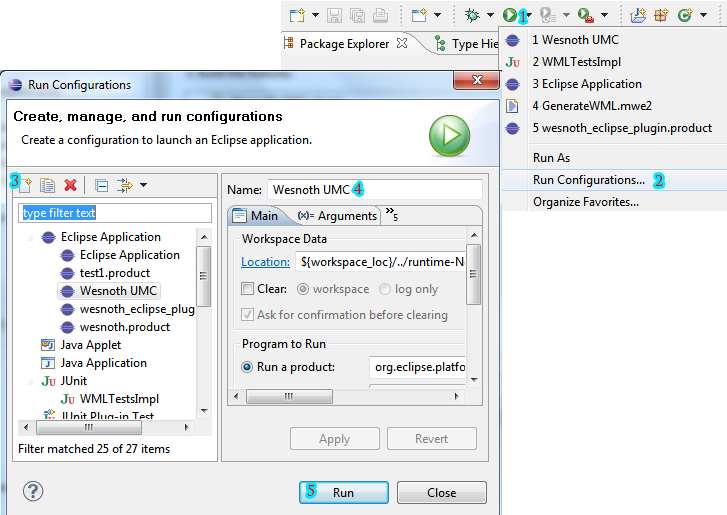
\includegraphics[scale=0.7]{launch_plugin.png}
\end{center}

\section{Frequently Asked Questions}
\subsection{Where can I submit any bugs found?}
Go over to Wesnoth's bug tracker: \href{https://gna.org/bugs/?func=additem&group=wesnoth&bug_group_id=116}{Add new bug}. Please be as specific as possible. Also, if you have any logs, please attach them.

\subsection{Why Mac OSX 32 bit is not supported?}
Apple decided to manage itself the versions that can run on each Mac version. Thus the modern Java SE6 version - which is used by the plugin - is not available on 32 bit Macs but on 64bit only. The 32bit Macs have just Java SE5 version available. Trying to port the plugin to the ``outdated" java version is not likely to be done, so please consider upgrading your OS.

\end{document}
